% 2008 年江西卷理科第 21 题：双曲线 x^2-y^2=1，点 P 在直线 x=m（0<m<1）上，过 P 的两条切线与双曲线
%   相切于 A、B，定点 M(1/m,0)；过 A 作直线 x-y=0 的垂线，垂足为 N。
% 来源 PDF：gaokaomath-src/普通高考/2008/2008江西理.pdf
% SHA-256：8d079d71fadf20911ed2fd71acfe9562b94eb962cfe5228fe7a376f3b599b239
% 原页：2008江西理.pdf 第 2 页（A3 三栏）第 2 栏，书页码 460。
% 绘制依据：取 m=1/2，P(1/2,-2)。切点弦为 mx-y0y=1，即 x/2+2y=1，与 x^2-y^2=1 交于
%   A(1.029,0.243)（右支上侧）与 B(-1.296,0.824)（左支上侧）；M(2,0)；
%   N 为 A 到直线 y=x 的垂足，N=((x_A+y_A)/2,(x_A+y_A)/2)=(0.636,0.636)。
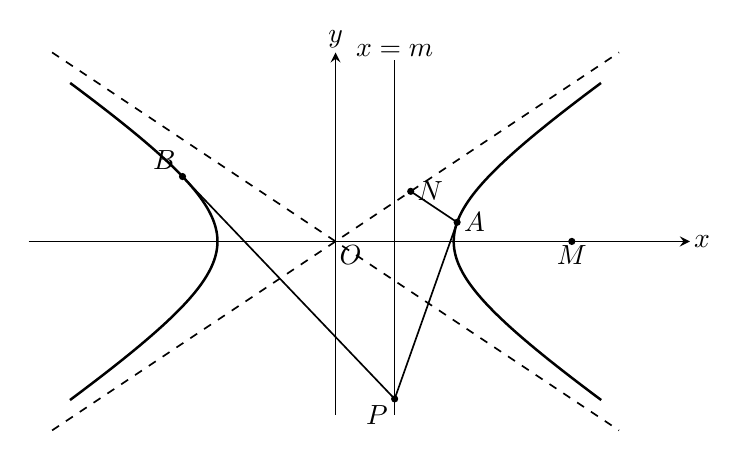
\begin{tikzpicture}[x=1.5cm, y=1.0cm, semithick, every node/.style={inner sep=1.2pt}]
  \draw[->,>=stealth] (-2.6,0) -- (3.0,0) node[right] {$x$};
  \draw[->,>=stealth] (0,-2.2) -- (0,2.4) node[above] {$y$};
  \node[below right] at (0,0) {$O$};

  % 渐近线
  \draw[dashed] (-2.4,-2.4) -- (2.4,2.4);
  \draw[dashed] (-2.4,2.4) -- (2.4,-2.4);

  % 双曲线两支
  \draw[line width=0.9pt, domain=-1.45:1.45, samples=80] plot ({cosh(\x)},{sinh(\x)});
  \draw[line width=0.9pt, domain=-1.45:1.45, samples=80] plot ({-cosh(\x)},{sinh(\x)});

  \coordinate (A) at (1.029,0.243);
  \coordinate (B) at (-1.296,0.824);
  \coordinate (P) at (0.5,-2);
  \coordinate (M) at (2,0);
  \coordinate (N) at (0.636,0.636);

  % 直线 x=m
  \draw (0.5,-2.2) -- (0.5,2.3);
  \node[above] at (0.5,2.3) {$x=m$};

  % 两条切线
  \draw (P) -- (A);
  \draw (P) -- (B);

  % A 到 y=x 的垂线，垂足 N
  \draw (A) -- (N);

  \fill (P) circle (1.3pt); \node[below left=1pt] at (P) {$P$};
  \fill (A) circle (1.3pt); \node[right=1pt] at (A) {$A$};
  \fill (B) circle (1.3pt); \node[above left=1pt] at (B) {$B$};
  \fill (M) circle (1.3pt); \node[below] at (M) {$M$};
  \fill (N) circle (1.3pt); \node[right=1pt] at (N) {$N$};
\end{tikzpicture}
